\scanpage{78}
est de rang fini: \inserted{(vérifier d'après cas décomposable)} (voir Chap I, \S~1, N\textsuperscript{o} 2, définition 1), et reste donc vraie par raison de continuité dans le cas général. Conjointement avec (13), on trouve

{\reversemarginpar\margin{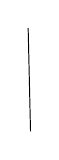
\begin{tikzpicture}[x=1cm,y=1cm]\draw[line width=.35pt] (0,0)--(.03,-1.31);\end{tikzpicture}}}
\uline{Corollaire 2} Sous les conditions précédentes, on a

\[
\begin{array}{@{}l@{\qquad}l@{}}
(15) & {\color{red}\boxed{{\color{black}\displaystyle |\alpha_n u_1,\mathord{-}u_n)|\leq\frac1{n!}\lVert u_1\rVert\mathord{-}\,\mathord{-}\lVert u_n\rVert}}}
\end{array}
\]

(Cela résulte aussi du fait, déjà signalé, que le coëfficient $k_n$ du Chap I, \S~1, N\textsuperscript{o} 2, prop 1, est ici égal à 1).

{\reversemarginpar\margin{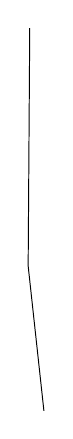
\begin{tikzpicture}[x=1cm,y=1cm]\draw[line width=.35pt] (0,0)--(-.02,-3.02)--(.18,-4.86);\end{tikzpicture}}}
\uline{Corollaire 3} Soit \deleted{$u\in L^1(E)$, où $E$ est un espace de Hilb} \inserted{$u$ un op. de Fredholm dans un} espace de Hilbert $E$. \deleted{Alors,} Si $u$ est un op. de Fredholm, il en est de même de $\overset{n}{\Lambda}u$, et on a

\[
\begin{array}{@{}l@{\qquad}l@{}}
(16) & \displaystyle \lVert\overset{n}{\Lambda}u\rVert_1=\alpha_n\deleted{\unsure{(\sqrt{u^*u})}}(|u|)\inserted{={\color{red}\underline{{\color{black}\alpha_n(\sqrt{\unsure{u^*u|u^*}})}}}}
\end{array}
\]

Si $u$ est un op. de H--S., il en est de même de $\overset{n}{\Lambda}u$, et on a

\[
\begin{array}{@{}l@{\qquad}l@{}}
(\unsure{17|14}) & \displaystyle \lVert\overset{n}{\Lambda}u\rVert_2=\sqrt{\alpha_n(u^*u)}
\end{array}
\]

On a, si $u\in L^1(E)$, $\lVert\overset{n}{\Lambda}u\rVert_1=\operatorname{Tr}\deleted{\sqrt{\vphantom{(\overset{n}{\Lambda}u)^*}}}\bigl((\overset{n}{\Lambda}u)^*(\overset{n}{\Lambda}u)\bigr)^{1/2}$ (N\textsuperscript{o} 1, formule (22)), or, (prop 1) on a $\deleted{\sqrt{\vphantom{(\overset{n}{\Lambda}u)^*}}}\bigl((\overset{n}{\Lambda}u)^*(\overset{n}{\Lambda}u)\bigr)^{1/2}=\overset{n}{\Lambda}\bigl((u^*u)^{1/2}\bigr)$, d'où \deleted{(16) en vertu de (17)} \inserted{$\lVert\overset{n}{\Lambda}u\rVert_1=\operatorname{Tr}\overset{n}{\Lambda}((u^*u)^{1/2})=\alpha_n(\sqrt{u^*u})$} (en vertu de (14)).

\deleted{Si $u\in L^2(E)$, \inserted{alors} on a encore, $(\overset{n}{\Lambda}u)^*(\overset{n}{\Lambda}u)=\overset{n}{\Lambda}(u^*u)$ \unsure{où on} \unsure{avait} $u^*u\in L^1(E)$ \inserted{est op. de Fredholm} (d'où $(\overset{n}{\Lambda}u)^*(\overset{n}{\Lambda}u)=\overset{n}{\Lambda}(u^*u)$ est $\in L^1(E)$, et $\overset{n}{\Lambda}u$ \unsure{par suite}}

Si $u$ est un op. de H.--S., alors $u^*u$ est un op. de Fredholm (N\textsuperscript{o} 1, th.~4), donc $(\overset{n}{\Lambda}u)^*(\overset{n}{\Lambda}u)=\overset{n}{\Lambda}(u^*u)$ est un op. de Fredholm, \deleted{et} donc $\overset{n}{\Lambda}u$ est un op. de H.--S. On a (N\textsuperscript{o} 1, th.~3, corollaire 3)

\[
(\lVert\overset{n}{\Lambda}u\rVert_2)^2=\operatorname{Tr}(\overset{n}{\Lambda}u)^*(\overset{n}{\Lambda}u)=\alpha_n(u^*u)\qquad\text{(formule (14), d'où (17))}
\]
{\reversemarginpar\margin{\unsure{79|75}}}
